% Project-authored dose-response measurements on a logarithmic dose axis.
% Syntax reference: https://tikz.dev/pgfplots/reference-axis
\documentclass{article}
\usepackage{pgfplots}
\pgfplotsset{compat=1.18}

\title{Dose-Response Pilot Study}
\author{Applied Biology Laboratory}
\date{September 2026}

\begin{document}
\maketitle

\section{Response across four orders of magnitude}
Two illustrative preparations were measured at seven positive doses. The
first reaches half of its observed maximum earlier; the second rises more
gradually. A logarithmic dose axis displays the low-dose region without
compressing the high-dose measurements into a single point.

\begin{figure}
\centering
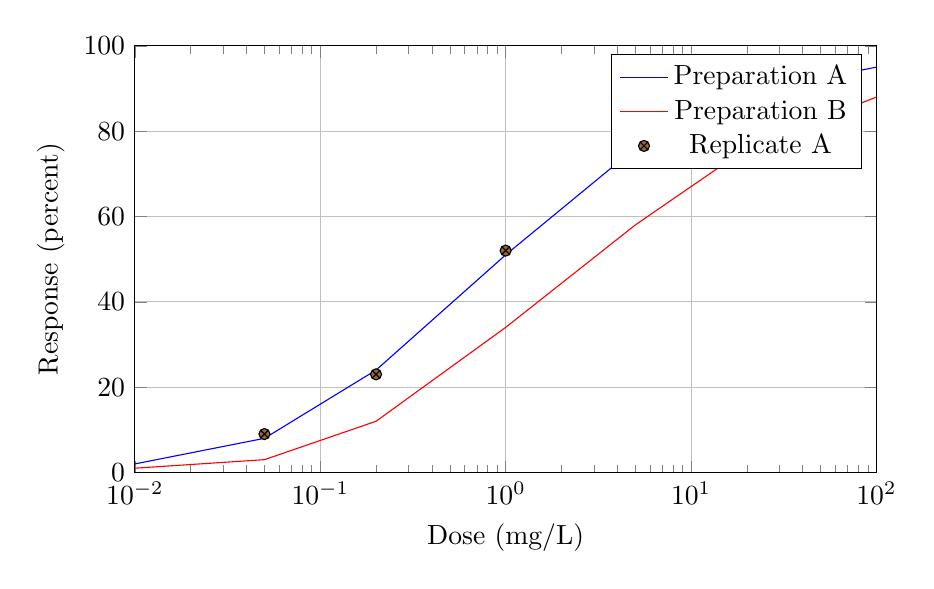
\begin{tikzpicture}
  \begin{semilogxaxis}[
    xmin=0.01,xmax=100,ymin=0,ymax=100,
    width=11cm,height=7cm,
    xlabel={Dose (mg/L)},ylabel={Response (percent)},grid=major]
    \addplot[blue] coordinates {
      (0.01,2) (0.05,8) (0.2,24) (1,51)
      (5,76) (20,89) (100,95)
    };
    \addlegendentry{Preparation A}
    \addplot[red] coordinates {
      (0.01,1) (0.05,3) (0.2,12) (1,34)
      (5,58) (20,76) (100,88)
    };
    \addlegendentry{Preparation B}
    \addplot+[black,only marks] coordinates {
      (0.05,9) (0.2,23) (1,52) (5,75) (20,90)
    };
    \addlegendentry{Replicate A}
  \end{semilogxaxis}
\end{tikzpicture}
\caption{Response profiles and selected replicate measurements.}
\label{fig:dose-response}
\end{figure}

All plotted doses are positive, as required by the logarithmic x-axis.
The dotted grid helps compare the two profiles at common dose levels.
\end{document}
